%% 04_results.tex
% Numbers from: analysis/results.md, analysis/recall_at_k.md,
%               analysis/latency_tokens.md, analysis/feature_extraction.md,
%               analysis/error_taxonomy.md

\section{Results}
\label{sec:results}

\subsection{Overall Accuracy}
\label{sec:results:overall}

% Source: analysis/results.md, Section 1
Table~\ref{tab:main_results} reports overall exact-match accuracy for all three systems
on the 13,800-question evaluation (N per system, fully paired by question\_id).
System~A (Narrative RAG) achieves 40.6\% exact-match (Wilson 95\%~CI [39.8\%, 41.4\%]),
outperforming System~B (Structured Naive) at 35.3\% [34.5\%, 36.1\%] and System~C
(Structured Aware) at 33.4\% [32.6\%, 34.2\%].

\begin{table}[!htbp]
\centering
\caption{Overall exact-match accuracy (N = 13,800 per system, fully paired).
Wilson 95\% CIs shown. Paired bootstrap differences and McNemar test statistics
are reported separately in Table~\ref{tab:pairwise}.}
\label{tab:main_results}
\begin{tabular}{lccc}
\toprule
System & Correct & Exact-match & Wilson 95\% CI \\
\midrule
A -- Narrative RAG & 5,600 & 40.6\% & [39.8\%, 41.4\%] \\
B -- Structured Naive & 4,873 & 35.3\% & [34.5\%, 36.1\%] \\
C -- Structured Aware & 4,605 & 33.4\% & [32.6\%, 34.2\%] \\
\bottomrule
\end{tabular}
\end{table}

% Source: analysis/results.md, Sections 2--3
All three pairwise differences are statistically significant.
Table~\ref{tab:pairwise} shows paired bootstrap confidence intervals and McNemar
test statistics; all bootstrap CIs exclude zero and all McNemar $p < 0.001$.

\begin{table}[!htbp]
\centering
\caption{Pairwise accuracy comparisons. Paired bootstrap (10,000 resamples, seed 42,
paired by question\_id). McNemar $\chi^2$ uses the uncorrected formula $(b-c)^2 / (b+c)$
with 1~df. Phi = effect size.}
\label{tab:pairwise}
\begin{tabular}{lccc}
\toprule
Comparison & Observed diff (pp) & Bootstrap 95\% CI & McNemar $\chi^2$ ($p$, $\phi$) \\
\midrule
A vs.\ B & +5.27 & [+4.5\%, +6.0\%] & 185.0 ($p{<}0.001$, $\phi{=}0.116$) \\
A vs.\ C & +7.21 & [+6.4\%, +8.0\%] & 330.8 ($p{<}0.001$, $\phi{=}0.155$) \\
B vs.\ C & +1.94 & [+1.3\%, +2.5\%] &  40.2 ($p{<}0.001$, $\phi{=}0.054$) \\
\bottomrule
\end{tabular}
\end{table}

The effect sizes (phi 0.054--0.155) are modest, consistent with a 5--7 percentage-point
absolute gap on a large, difficult question set.  We return to their practical significance
in Section~\ref{sec:discussion}.

Figure~\ref{fig:partial_vs_exact} compares partial-credit and exact-match scores at the
system $\times$ family level.  Almost every cell sits on or above the identity line,
indicating that wrong answers are usually \emph{near-miss} rather than entirely off-target.
The largest gap above the diagonal is for System~C on temporal\_comparison
(exact 0.34, partial 0.43), confirming that resource-aware retrieval often gets within
a tolerance of the correct date even when exact-match fails.

\begin{figure}[!htbp]
\centering
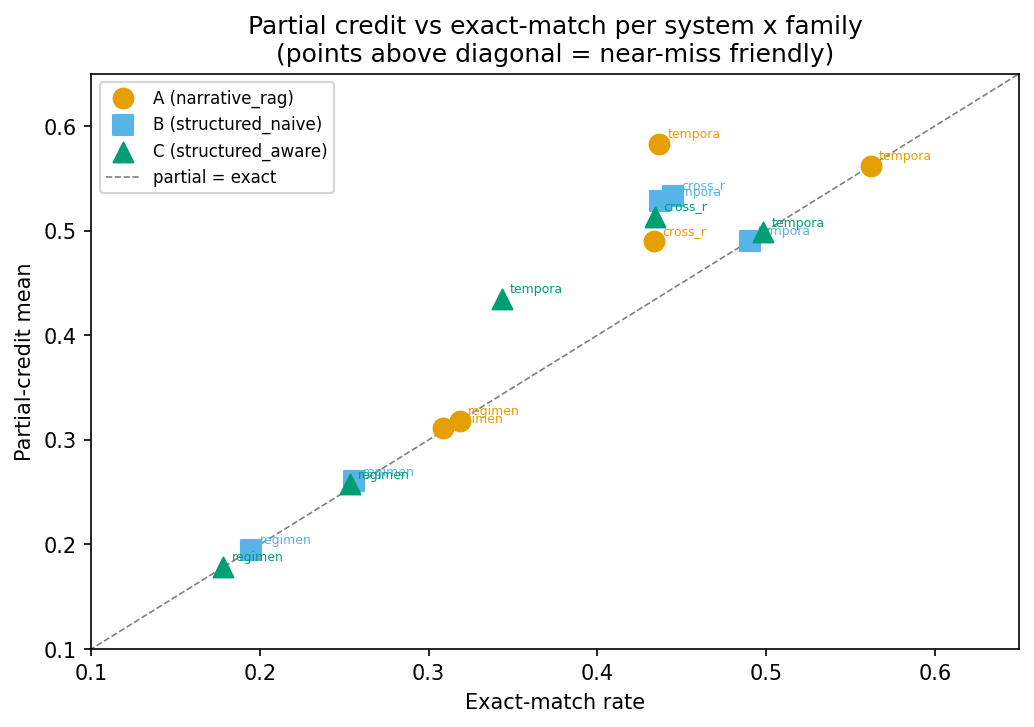
\includegraphics[width=0.75\textwidth]{figures/partial_vs_exact.png}
\caption{Partial-credit (with type-specific tolerance) vs.\ exact-match per
system $\times$ question family.  Points above the diagonal indicate that partial-credit
recovers near-misses that exact-match does not.  System~C on temporal\_comparison is the
clearest case where the system gets close to the correct date without matching exactly.}
\label{fig:partial_vs_exact}
\end{figure}

\subsection{Complexity Gradient}
\label{sec:results:tiers}

% Source: analysis/results.md, Section 5
Figure~\ref{fig:accuracy_by_tier} plots accuracy by tier for all three systems.
A sharp complexity gradient is observed across all systems: Tier~1 accuracy is
approximately 41--54\% while Tier~3 collapses uniformly to approximately 20\% regardless
of retrieval architecture.

\begin{table}[!htbp]
\centering
\caption{Accuracy by complexity tier (Wilson 95\% CIs).
Tier 1: single LAI on fixed schedule; Tier 2: cyclic regimen; Tier 3: multi-drug.}
\label{tab:tier_results}
{\small
\setlength{\tabcolsep}{4pt}
\begin{tabular}{lccccccc}
\toprule
Tier & $n$ & A acc & A 95\% CI & B acc & B 95\% CI & C acc & C 95\% CI \\
\midrule
1 & 4,347 & 53.9\% & [52.4\%, 55.3\%] & 47.0\% & [45.5\%, 48.5\%] & 40.8\% & [39.3\%, 42.2\%] \\
2 & 4,347 & 51.0\% & [49.5\%, 52.5\%] & 41.8\% & [40.4\%, 43.3\%] & 41.6\% & [40.2\%, 43.1\%] \\
3 & 5,106 & 20.4\% & [19.3\%, 21.6\%] & 19.8\% & [18.7\%, 20.9\%] & 20.1\% & [19.0\%, 21.2\%] \\
\bottomrule
\end{tabular}
}
\end{table}

% Source: analysis/results.md, Section 5 monotonicity notes
Systems A and B show monotone decline (A: 53.9\% $>$ 51.0\% $>$ 20.4\%; B: 47.0\%
$>$ 41.8\% $>$ 19.8\%).  System~C shows a non-monotone pattern at Tiers~1--2
(40.8\% at Tier~1, 41.6\% at Tier~2), consistent with the resource-aware retriever
providing more benefit on cyclic multi-component questions than on simple single-LAI
lookups.  Tier~3 convergence to $\approx 20\%$ across all systems indicates that
hard temporal arithmetic (multi-drug staggered schedules) is not solved by any of
the three retrieval architectures at the current answer budget.

\subsection{By Question Family}
\label{sec:results:families}

% Source: analysis/results.md, Section 4
Table~\ref{tab:family_results} reports accuracy by question family.

\begin{table}[!htbp]
\centering
\caption{Accuracy by PSP adherence-indicator family (Wilson 95\% CIs).}
\label{tab:family_results}
{\small
\setlength{\tabcolsep}{4pt}
\begin{tabular}{lccccccc}
\toprule
Family & $n$ & A acc & A 95\% CI & B acc & B 95\% CI & C acc & C 95\% CI \\
\midrule
temporal\_lookup   & 3,200 & 56.2\% & [54.5\%, 57.9\%] & 49.0\% & [47.3\%, 50.8\%] & 49.8\% & [48.1\%, 51.6\%] \\
temporal\_comparison & 2,400 & 43.7\% & [41.7\%, 45.7\%] & 43.7\% & [41.7\%, 45.7\%] & 34.3\% & [32.5\%, 36.3\%] \\
cross\_resource    & 1,600 & 43.4\% & [41.0\%, 45.8\%] & 44.5\% & [42.1\%, 46.9\%] & 43.4\% & [41.0\%, 45.9\%] \\
regimen\_compliance & 4,200 & 30.9\% & [29.5\%, 32.3\%] & 25.6\% & [24.3\%, 26.9\%] & 25.3\% & [24.0\%, 26.6\%] \\
regimen\_aggregation & 2,400 & 31.8\% & [30.0\%, 33.7\%] & 19.5\% & [18.0\%, 21.1\%] & 17.8\% & [16.4\%, 19.4\%] \\
\bottomrule
\end{tabular}
}
\end{table}

Two findings stand out.  The cross\_resource family is at parity across all three systems
(A=43.4\%, B=44.5\%, C=43.4\%), indicating that the advantage of structured or
resource-aware retrieval does not emerge on multi-resource relational questions at this
difficulty level, at least within the current answer budget.  The narrative advantage is
largest on regimen\_aggregation (A leads B by 12.3~pp; bootstrap CI excludes zero) and
regimen\_compliance (A leads B by 5.3~pp), reflecting that FHIR JSON serialisation
imposes a context-length cost that hurts dose-count arithmetic.  Figure~\ref{fig:heatmap}
visualises the same comparison and makes the family-level patterns easier to scan.

\begin{figure}[!htbp]
\centering
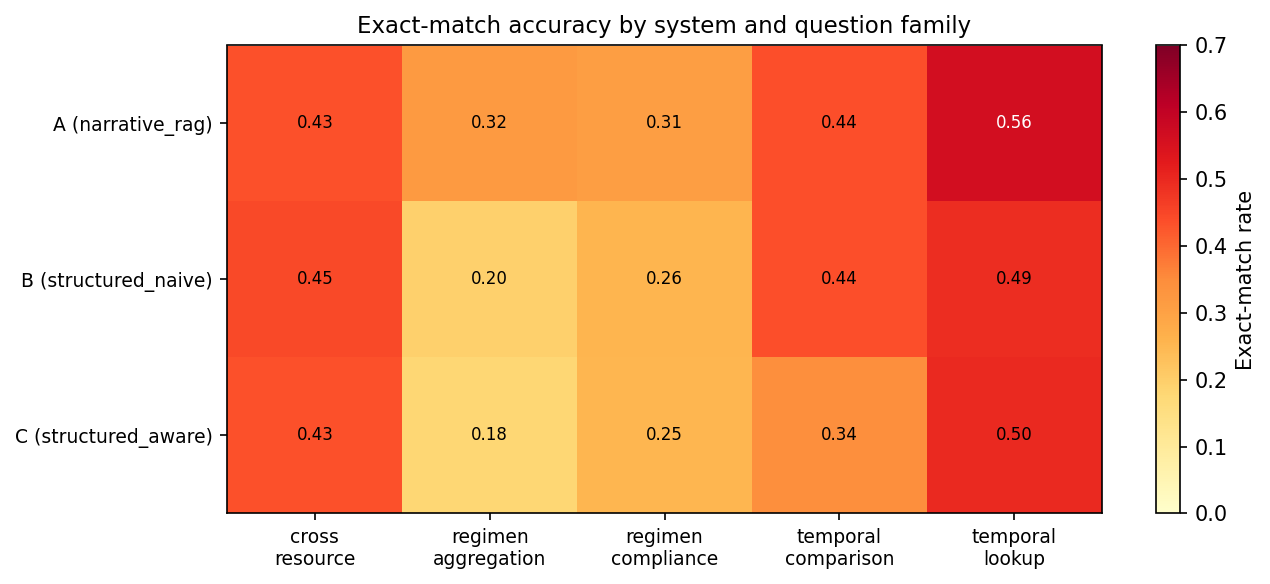
\includegraphics[width=0.85\textwidth]{figures/accuracy_heatmap.png}
\caption{Exact-match accuracy by system (rows) and PSP question family (columns).
The brightest column (temporal\_lookup) is where all three systems perform best, while
the dimmest cells (regimen\_aggregation and regimen\_compliance under structured systems)
mark the largest narrative advantage.  cross\_resource is near-uniform across systems.}
\label{fig:heatmap}
\end{figure}

\subsection{Retrieval Recall vs.\ Answer Accuracy}
\label{sec:results:recall}

% Source: analysis/recall_at_k.md
System~A recall@k is N/A: narrative chunks carry no FHIR resource IDs and a
resource-level recall cannot be defined.  For Systems~B and~C, Table~\ref{tab:recall}
shows overall recall@5.

\begin{table}[!htbp]
\centering
\caption{Retrieval recall@k (B vs.\ C). System~A = N/A (no FHIR resource IDs on
narrative chunks). Values shown as mean recall [Wilson 95\% CI mean across strata].}
\label{tab:recall}
{\small
\setlength{\tabcolsep}{4pt}
\begin{tabular}{lcccc}
\toprule
System & $k=1$ & $k=3$ & $k=5$ & $k=10$ \\
\midrule
B -- Structured Naive  & 0.573 [0.543, 0.602] & 0.739 [0.711, 0.765] & 0.762 [0.735, 0.787] & 0.762 [0.735, 0.787] \\
C -- Structured Aware  & 0.664 [0.636, 0.690] & 0.829 [0.807, 0.848] & 0.852 [0.831, 0.870] & 0.852 [0.831, 0.870] \\
\bottomrule
\end{tabular}
}
\end{table}

System~C retrieves the relevant resource more often than System~B at $k=1$ (0.664 vs.\
0.573) and $k=5$ (0.852 vs.\ 0.762).  The $k=1$ gap confirms that the resource-aware
primitives (typed filter, reference traversal, temporal pre-filter) correctly rank the
relevant resource higher.  Figure~\ref{fig:recall_at_k} shows the recall curves stratified
by complexity tier; the $k=1$ advantage of C over B is largest at Tier~3 (0.53 vs.\ 0.42),
where multi-drug staggered schedules make naive dense retrieval least reliable.
However, this retrieval advantage \emph{does not translate into an end-to-end accuracy
advantage}: C scores 33.4\% exact-match vs.\ B's 35.3\%.  The most likely explanation
is that the FHIR-JSON context fed to the answer LLM remains harder to reason over
than narrative text, even when the correct resource is retrieved.

\begin{figure}[!htbp]
\centering
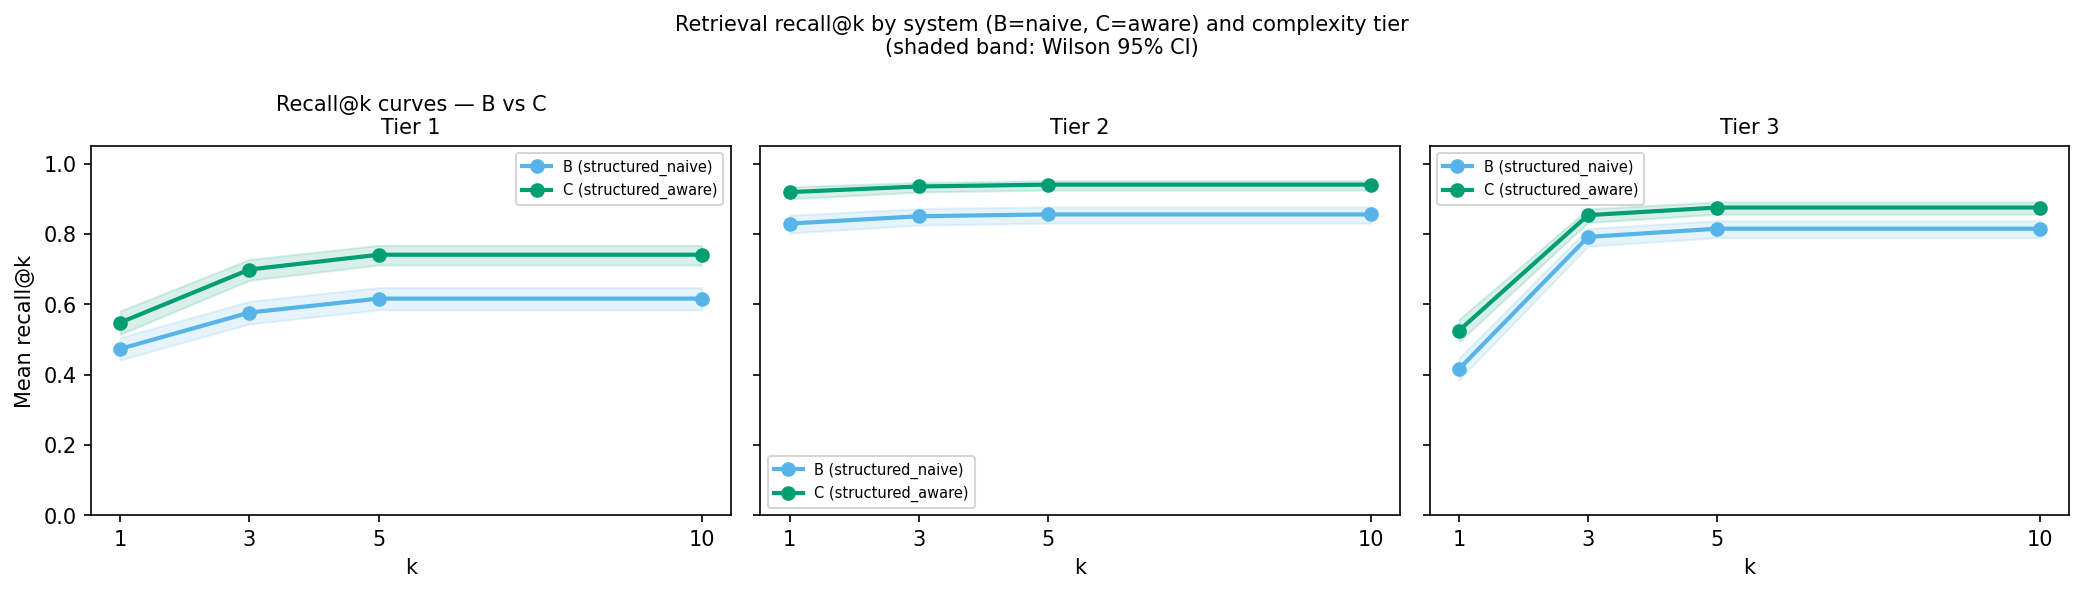
\includegraphics[width=0.95\textwidth]{figures/recall_at_k_curve.png}
\caption{Retrieval recall@$k$ for Systems~B (Structured Naive) and C (Structured Aware)
stratified by complexity tier.  Shaded band: Wilson 95\%~CI.  System~C dominates
System~B at every $k$ and tier; the gap is largest at $k=1$, confirming that the
resource-aware primitives rank the correct FHIR resource higher rather than merely
recalling it.  System~A is omitted because narrative chunks carry no FHIR resource IDs.}
\label{fig:recall_at_k}
\end{figure}

\subsection{Latency, Tokens, and Cost}
\label{sec:results:latency}

% Source: analysis/latency_tokens.md
Table~\ref{tab:latency} summarises latency and token usage.

\begin{table}[!htbp]
\centering
\caption{Latency (milliseconds) and mean token usage per call.
Cost computed at Groq Developer-plan rates (\$0.29/M tokens-in, \$0.59/M tokens-out)
applied to total tokens consumed in the evaluation run.}
\label{tab:latency}
\begin{tabular}{lccccc}
\toprule
System & p50 (ms) & p95 (ms) & p99 (ms) & Tokens-in (mean) & Cost (USD) \\
\midrule
A -- Narrative  & 1,060 & 6,031  & 53,038 &   490 & \$4.74 \\
B -- Naive      & 1,354 & 17,890 & 46,301 & 4,463 & \$21.07 \\
C -- Aware      & 1,056 & 4,538  &  8,513 & 2,175 & \$6.88 \\
\bottomrule
\end{tabular}
\end{table}

System~B's 9$\times$ context expansion (4,463 vs.\ 490 mean tokens-in) drives a
4.4$\times$ cost premium over System~A (\$21.07 vs.\ \$4.74) and the highest
tail latency (p99 = 46,301~ms).  System~C's resource-aware filtering reduces context
by approximately 51\% vs.\ B, yielding the lowest p50 latency (1,056~ms) and a cost
of \$6.88, well below B and 1.5$\times$ A.  Total compute cost across all three
systems was \$32.68 at list-price token rates over live (non-cached) calls; the
actual billed amount was lower because of response-cache reuse during reproducible
re-runs.  Neither structured system is cost-effective relative to System~A given
the accuracy deficit at the current 512-token answer budget.

\subsection{Error Taxonomy}
\label{sec:results:errors}

% Source: analysis/error_taxonomy.md
Figure~\ref{fig:error_taxonomy} and Table~\ref{tab:errors} show the distribution of
failure modes across a stratified sample of 50 failures per system (10 per family, seed 42).

\begin{table}[!htbp]
\centering
\caption{Error taxonomy distribution (n=50 per system, stratified by family).
Seed = 42. Single-rater classification by deterministic regex rules.}
\label{tab:errors}
\begin{tabular}{lcccccc}
\toprule
Category & A ($n$) & A (\%) & B ($n$) & B (\%) & C ($n$) & C (\%) \\
\midrule
Reasoning-truncated       & 22 & 44\% & 29 & 58\% & 26 & 52\% \\
Temporal-anchor failure   & 15 & 30\% & 9  & 18\% & 5  & 10\% \\
N/A misuse                & 4  & 8\%  & 7  & 14\% & 11 & 22\% \\
Wrong-entity / enum       & 5  & 10\% & 3  & 6\%  & 6  & 12\% \\
Other / unclassified      & 4  & 8\%  & 2  & 4\%  & 2  & 4\%  \\
\midrule
\textbf{Total}            & \textbf{50} & & \textbf{50} & & \textbf{50} & \\
\bottomrule
\end{tabular}
\end{table}

Reasoning truncation is the dominant failure mode across all three systems (44--58\%),
reflecting the 512-token output budget.  The rate is highest for B (58\%) and C (52\%)
because FHIR-JSON contexts require longer chain-of-thought arithmetic before a final answer
can be stated; the same LLM, given the same reasoning task, runs out of budget sooner when
the context is denser.  This is a token-budget artefact, not an architectural property of
narrative vs.\ structured retrieval.

Temporal-anchor failures follow a gradient: 30\% for A, 18\% for B, 10\% for C.
Narrative chunks do not embed the question's reference date (a per-question parameter, not
a feature of the narrative text), so the LLM must infer the temporal anchor from context.
FHIR resources (\texttt{CarePlan.period.start/end}, \texttt{MedicationAdministration.effectiveDateTime})
provide explicit date fields from which a temporal anchor can sometimes be inferred,
explaining the lower rate for B and C.

N/A misuse increases from A (8\%) to C (22\%): structured systems retrieve FHIR components
directly, making it more likely that the model encounters records for absent components
(Tier-1 patients have no adjunct or rescue component) and computes a phantom value rather
than returning N/A.

\subsection{Feature-Extraction Arm (O6)}
\label{sec:results:o6}

% Source: analysis/feature_extraction.md
Table~\ref{tab:auc} reports AUC-ROC for the synthetic adherence classification task
(label: $\geq$2 consecutive missed doses in final 60~d OR median gap $>$ 1.5$\times$
prescribed interval in final 90~d; class balance 14.5\% positive / 85.5\% negative;
200 patients; 5-fold stratified CV).

\begin{table}[!htbp]
\centering
\caption{Feature-extraction arm AUC-ROC (Objective O6). Bootstrap 95\% CIs at patient
level from out-of-fold predictions (10,000 resamples). FS-Structured = FHIR-derived
numerics; FS-Narrative = heuristic regex on LLM narratives; FS-Aware = per-patient
aggregates from System~C retrieval traces.}
\label{tab:auc}
\begin{tabular}{lcc}
\toprule
Feature set & LightGBM AUC & Logistic Regression AUC \\
\midrule
FS-Structured & 0.997 [0.986, 1.000] & 1.000 [0.999, 1.000] \\
FS-Narrative  & 0.843 [0.771, 0.896] & 0.836 [0.764, 0.897] \\
FS-Aware      & 0.793 [0.680, 0.865] & 0.708 [0.634, 0.799] \\
\bottomrule
\end{tabular}
\end{table}

\begin{figure}[!htbp]
\centering
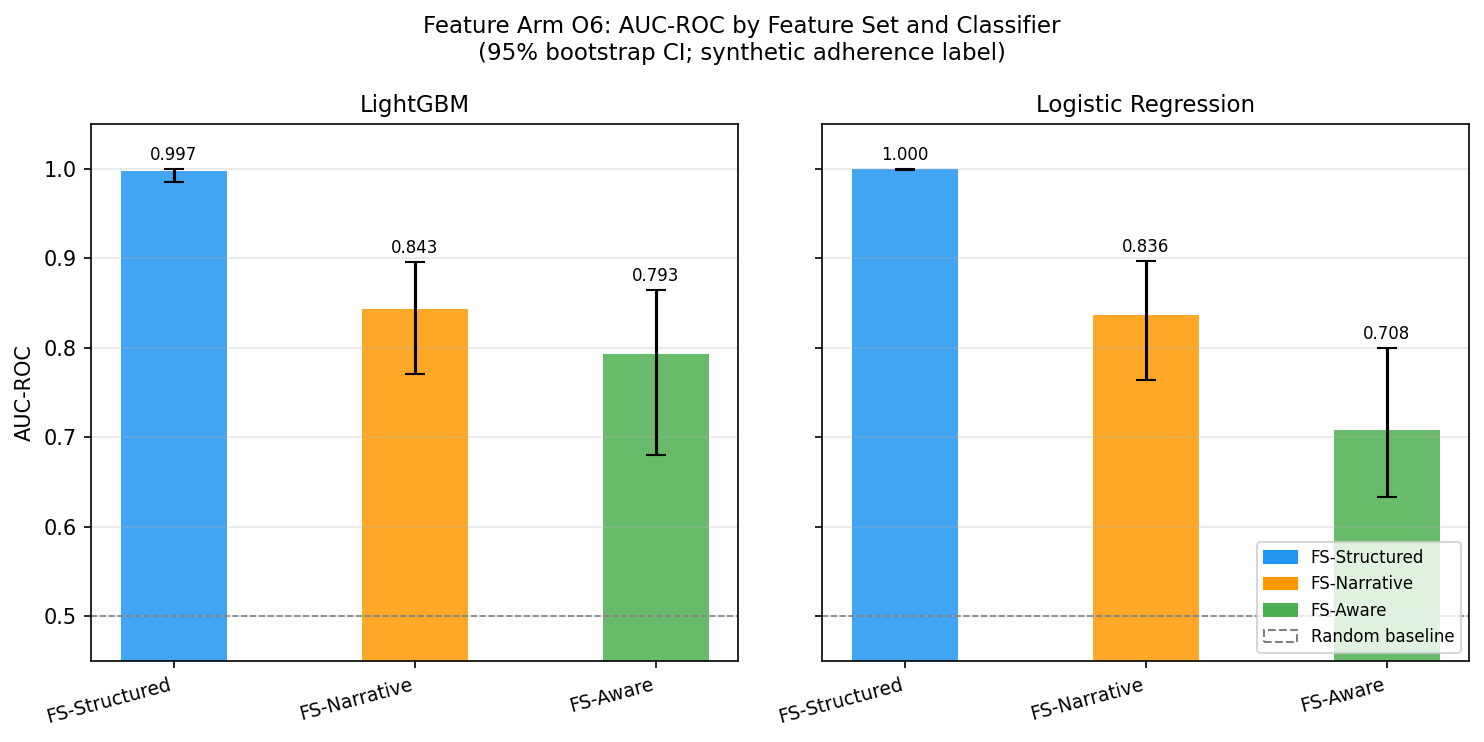
\includegraphics[width=0.95\textwidth]{figures/feature_arm_auc.png}
\caption{Feature-arm AUC-ROC by feature set and classifier (LightGBM, left;
logistic regression, right).  Error bars are 95\% bootstrap CIs at the patient level.
FS-Structured features outperform both FS-Narrative and FS-Aware by a wide margin under
both classifiers.  The near-ceiling FS-Structured AUC is partly attributable to
feature-label alignment in the synthetic adherence label and is discussed in
Section~\ref{sec:results:o6}.}
\label{fig:feature_auc}
\end{figure}

% Source: analysis/feature_extraction.md, pairwise differences
Pairwise bootstrap differences (LightGBM): FS-Structured vs.\ FS-Narrative
$\Delta{=}+0.160$ [+0.099, +0.226]; FS-Structured vs.\ FS-Aware $\Delta{=}+0.219$
[+0.132, +0.316]; FS-Narrative vs.\ FS-Aware $\Delta{=}+0.060$ [$-0.051$, $+0.177$].
The FS-Narrative vs.\ FS-Aware CI straddles zero: these two feature sets are tied
within the bootstrap interval.

% Source: analysis/feature_extraction.md, interpretation note
The near-perfect FS-Structured AUC (0.997--1.000) is partly a synthetic-data
artefact: the positive label is concentrated entirely in Tier-2 patients (all 29
positives are Tier~2; no Tier-1 or Tier-3 patient is labelled positive in this
perfectly-scheduled synthetic dataset).  FS-Structured features encode tier as one-hot
columns and directly capture the cyclic off-period gap via \texttt{gap\_max\_90d} and
\texttt{n\_events\_60d}.  FS-Narrative captures tier through ``tier~2'' / ``T2''
text patterns; FS-Aware captures it through the retrieval distribution.
The relative ordering (Structured $\gg$ Narrative $\approx$ Aware) and the CI widths
are signals about information richness under these feature extraction strategies,
even if the absolute AUC values are inflated by the synthetic-label structure.
Readers should not extrapolate the FS-Structured ceiling to real-world noisy adherence
data.

\begin{figure}[!htbp]
\centering
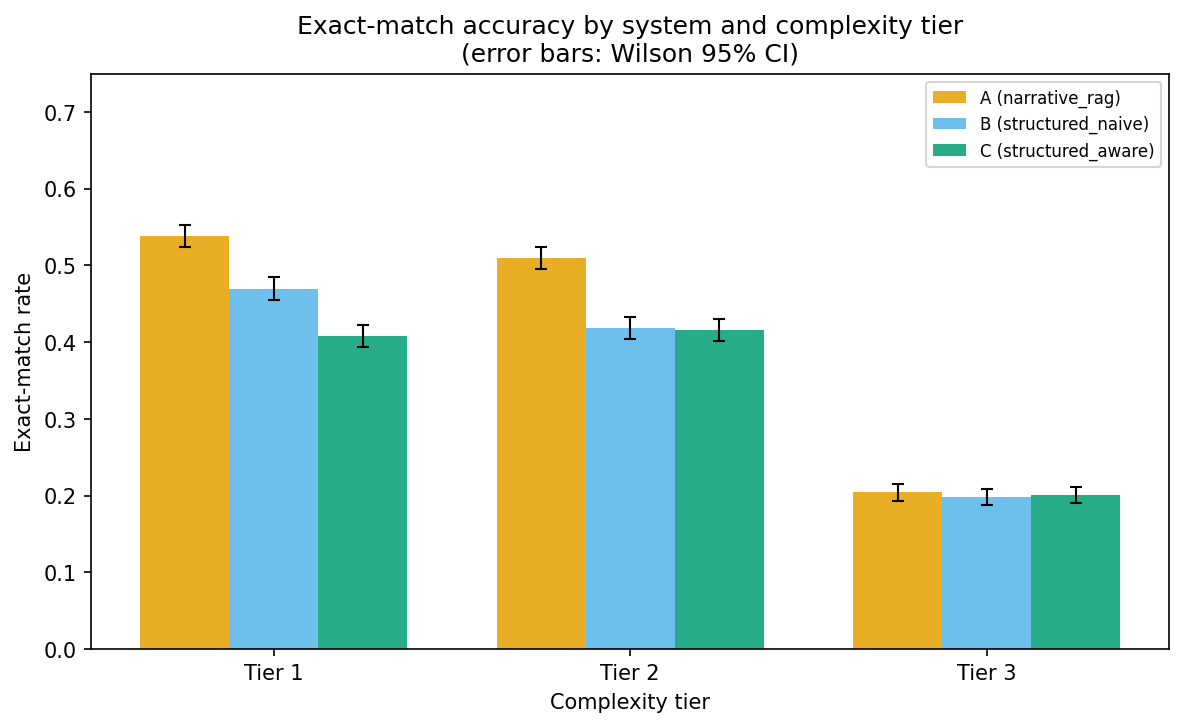
\includegraphics[width=0.85\textwidth]{figures/accuracy_by_tier.png}
\caption{Exact-match accuracy by system and complexity tier (Wilson 95\% CI error bars).
Tier~1: single long-acting injectable; Tier~2: cyclic regimen; Tier~3: multi-drug.
All three systems converge near 20\% at Tier~3, demonstrating that hard temporal
arithmetic over multi-drug schedules is not solved by any retrieval architecture
at the 512-token output budget.}
\label{fig:accuracy_by_tier}
\end{figure}

\begin{figure}[!htbp]
\centering
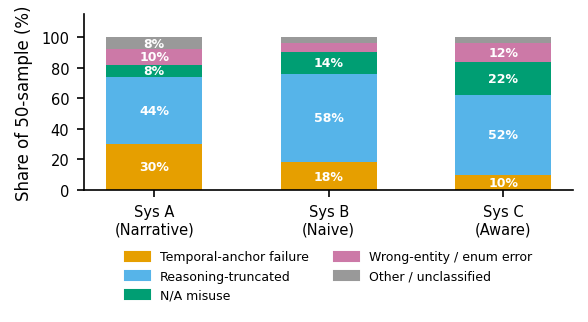
\includegraphics[width=0.85\textwidth]{figures/error_taxonomy_distribution.png}
\caption{Error category distribution across the stratified failure sample
(n=50 per system, seed=42; colours: Wong 2011 colorblind-safe palette).
Reasoning truncation (dark blue) is the single largest category for all three systems.
Temporal-anchor failures (orange) are highest for System~A, declining across B and C.}
\label{fig:error_taxonomy}
\end{figure}
